\documentclass[
	12pt,
	a4paper,
	BCOR10mm,
	%chapterprefix,
	DIV14,
	headsepline,
	usegeometry,
	%twoside,
	%openright
]{scrreprt}

\KOMAoptions{
	listof=totoc,
	bibliography=totoc,
	index=totoc
}

\usepackage[T1]{fontenc}
\usepackage[utf8]{inputenc}

\usepackage{lmodern}

\usepackage[ngerman,english]{babel}

\usepackage[toc]{appendix}
\usepackage{color}
\usepackage{eurosym}
\usepackage{fancyhdr}
\usepackage{geometry}
\usepackage{graphicx}
\usepackage[htt]{hyphenat}
\usepackage{listings}
\usepackage{lstautogobble}
\usepackage{microtype}
\usepackage[list=true,hypcap=true]{subcaption}
\usepackage{textcomp}
\usepackage{units}

\usepackage{varioref}
\usepackage[hidelinks]{hyperref}
\usepackage[capitalise,noabbrev]{cleveref}

\definecolor{uhhred}{cmyk}{0,1,1,0}


\usepackage{todonotes}
\usepackage{silence}
\WarningFilter{latex}{Marginpar} 
\WarningFilter{latexfont}{Font shape}
\WarningFilter{latexfont}{Some font}
\usepackage{changes}
\usepackage{lmodern}


\lstset{
	basicstyle=\ttfamily,
	frame=single,
	numbers=left,
	language=C,
	breaklines=true,
	breakatwhitespace=true,
	postbreak=\hbox{$\hookrightarrow$ },
	showstringspaces=false,
	autogobble=true,
	upquote=true,
	tabsize=4,
	captionpos=b,
	morekeywords={int8_t,uint8_t,int16_t,uint16_t,int32_t,uint32_t,int64_t,uint64_t,size_t,ssize_t,off_t,intptr_t,uintptr_t,mode_t}
}

\makeatletter
\renewcommand*{\lstlistlistingname}{List of Listings}
\makeatother

\begin{document}

\newgeometry{left=2cm, top=2cm, right=2cm, bottom=2cm}

\begin{titlepage}
	
\includegraphics[width=0.5\textwidth]{UHH-Logo_2010_Farbe_CMYK}

	\begin{center}
		{\Large \textcolor{uhhred}{\textbf{Projektbericht}}\par}

		\vspace{1cm}

		{\titlefont\huge Gaming AI\par}

		\vspace{1cm}

		{\large vorgelegt von\par}

		\vspace{0.5cm}

		{\large Friedrich Braun\\
				Valentin Krön\par}
	\end{center}

	\vfill

	{\large\noindent\begin{tabular}{l}
		Fakultät für Mathematik, Informatik und Naturwissenschaften\\
		Fachbereich Informatik\\
		Arbeitsbereich Wissenschaftliches Rechnen
	\end{tabular}\par}

	\vspace{1cm}

	{\large\noindent\begin{tabular}{lll}
		Studiengang:    & Wirtschaftsinformatik & Informatik \\
		Matrikelnummer: & 6252218 & 6700970 \\
		\\
		Betreuer:       & Eugen Betke & Julian Kunkel \\
		\\
		Hamburg, 2017-01-01
	\end{tabular}\par}
\end{titlepage}

\restoregeometry

\chapter*{Abstract}

\thispagestyle{empty}

Lorem ipsum dolor sit amet, consetetur sadipscing elitr, sed diam nonumy eirmod tempor invidunt ut labore et dolore magna aliquyam erat, sed diam voluptua.
At vero eos et accusam et justo duo dolores et ea rebum.
Stet clita kasd gubergren, no sea takimata sanctus est Lorem ipsum dolor sit amet.
Lorem ipsum dolor sit amet, consetetur sadipscing elitr, sed diam nonumy eirmod tempor invidunt ut labore et dolore magna aliquyam erat, sed diam voluptua.
At vero eos et accusam et justo duo dolores et ea rebum.
Stet clita kasd gubergren, no sea takimata sanctus est Lorem ipsum dolor sit amet.

\tableofcontents

\chapter{Einleitung}
\label{Einleitung}

\textit{%
In this chapter, ...
}

\bigskip

Lorem ipsum dolor sit amet, consetetur sadipscing elitr, sed diam nonumy eirmod tempor invidunt ut labore et dolore magna aliquyam erat, sed diam voluptua.
At vero eos et accusam et justo duo dolores et ea rebum.
Stet clita kasd gubergren, no sea takimata sanctus est Lorem ipsum dolor sit amet.
Lorem ipsum dolor sit amet, consetetur sadipscing elitr, sed diam nonumy eirmod tempor invidunt ut labore et dolore magna aliquyam erat, sed diam voluptua.
At vero eos et accusam et justo duo dolores et ea rebum.
Stet clita kasd gubergren, no sea takimata sanctus est Lorem ipsum dolor sit amet.\footnote{I am a footnote.}

Lorem ipsum dolor sit amet, consetetur sadipscing elitr, sed diam nonumy eirmod tempor invidunt ut labore et dolore magna aliquyam erat, sed diam voluptua.
At vero eos et accusam et justo duo dolores et ea rebum.
Stet clita kasd gubergren, no sea takimata sanctus est Lorem ipsum dolor sit amet:

\begin{itemize}
	\item Lorem
	\item Ipsum
\end{itemize}

Lorem ipsum dolor sit amet, consetetur sadipscing elitr, sed diam nonumy eirmod tempor invidunt ut labore et dolore magna aliquyam erat, sed diam voluptua.
At vero eos et accusam et justo duo dolores et ea rebum.
“Stet clita kasd gubergren, no sea takimata sanctus est Lorem ipsum dolor sit amet.”~\cite{Quelle2012}

\medskip

%Reference example: For more information, see
%\begin{itemize}
%  \item Chapter~\ref{Assignment},
%  \item \cref{Assignment},
%  \item \vref{Assignment}.
%\end{itemize}

\chapter{Projektziel}
\label{Projektziel}

\textit{%
In diesem Kapitel gehen wir auf das Projektziel näher ein und erläutern warum wir das Projektziel ändern mussten.
}

\bigskip

\section{Ursprüngliches Projektziel}

Unser ursprüngliches Projektziel bestand darin eine AI zu entwickeln und diese mit Hilfe eines genetischen Algorithmus zu trainieren. Diese AI sollte auf die Spring-RTS-Engine [Spring] angewandt werden. Die Absicht bestand darin zu zeigen, dass eine AI auf diese Weise lernen kann RTS-Spiele gut, eventuell sogar besser als menschliche Spieler, zu spielen.\\

\section{Gründe Für die Änderung des Projektziels}
Bei der Realisierung dieser Zielsetzung trafen wir allerdings auf unlösbare Probleme. Eines der Probleme lag im unübersichtlichen Aufbau der Spring-Engine [Spring] selbst. Zwar bietet die Spring-Engine eine Lobby an, jedoch lassen sich nur wenige Spiele tatsächlich starten und selbst bei diesen lassen sich keine externen AI's einbinden. Dadurch fehlte uns eine Vorlage, auf der wir unsere AI hätten aufbauen können; insbesondere fehlte uns Wissen zu den Schnittstellen zwischen unserer AI und der Spring-Engine [Spring]. \\
Einige Spiele haben im Code für das Spiel direkt eingebundene AI's, die auch lauffähig sind. Diese AI's halfen uns jedoch auch nicht weiter, gerade da sie direkt ins Spiel hineinkompiliert sind. Dies bedeutet nämlich nicht nur, dass die AI selber kaum zu Debuggen ist, man muss auch direkt am Spiel selber mit der Sprache lua arbeiten. Da die Auseinandersetzung mit dem Aufbau eines Spieles für die Spring-Engine und mit der Sprache lua den Projektrahmen gesprengt hätte, entschieden wir uns für eine Änderung der Zielsetzung.

\section{Neues Projektziel}
Da eine AI für die Spring-Engine selber nicht möglich war, beschlossen wir eine Simulation, also eine vereinfachte Version eines Spiels auf Basis der Spring-Engine, zu bauen. Wichtig ist bei unserem neuen Ziel vor allem ein ''proof-of-concept'', sprich: Wir wollen zeigen, dass es möglich ist eine AI für ein RTS zu bauen und diese mit Hilfe eines genetischen Algorithmus zu trainieren.


\chapter{Aufbau}
\label{Aufbau}

\textit{%
In diesem Kapitel beschreiben wir kurz den Aufbau der wichtigsten Bausteine des Projekts.
}

\bigskip

\section{Aufbau der Simulation}
Die Simulation ist ein sehr einfaches RTS. Sie ist ausgelegt auf genau zwei Spieler. Jeder der Spieler hat ein Hauptgebäude, dass in regelmäßigen Zeitabständen Einheiten erstellt. Diese Einheiten können zu Positionen auf dem Spielfeld laufen und, wenn sie dicht genug dran sind, Schaden an gegnerischen Einheiten verursachen. Fallen die Lebenspunkte einer Einheit auf null, so wird diese gelöscht.\\
Es gibt genau einen Einheitentyp. Die Simulation beinhaltet keinerlei Mechaniken, die Ressourcen in irgendeiner Form verwenden.\\
Ein Match dauert zehn Minuten.

\section{Aufbau der AI}
Da bei einem RTS die Anzahl der Einheiten, und damit die Anzahl der Möglichkeiten, variabel ist, entschieden wir uns, auch durch Anraten der Betreuer, dafür, die AI als Schwarmintelligenz zu designen.\\
Jede Einheit hat einen Sichtradius und gibt diese Information als Input an die AI. Diese wiederum generiert daraus über ein neuronales Netz eine Entscheidung. Damit verhalten sich alle Einheiten gleich bei gleicher Eingabe. \\
Durch den Aufbau als Schwarmintelligenz ist die AI problemlos skalierbar. Zudem benötigen wir keinerlei Koordination der Einheiten, da diese sich aus der Schwarmintelligenz von alleine ergibt.

\section{Aufbau des Trainingsalgorithmus}
Das Training der AI erfolgt dadurch, dass das neuronale Netz trainiert wird. Im Detail heißt das: Wir verwenden die Gewichte des neuronalen Netzes als Gene in einem genetischen Algorithmus. Dabei müssen wir nicht zwischen Geno- und Phänotyp unterscheiden. Die Rekombination erfolgt über einen zufälligen Schnitt. Die Mutation findet mit einer gewissen Wahrscheinlichkeit statt, wenn sie stattfindet so wird genau ein Gen durch ein zufälliges neues ersetzt.\\
Der Fitnesswert basiert auf der Anzahl lebender Einheiten, eigener wie gegnerischer, bei Spielende. Die genaue Umsetzung haben wir zu Auswertungszwecken variiert, weswegen wir in der Auswertung auch noch einmal genauer darauf eingehen.

\chapter{Umsetzung}
\label{Umsetzung}

\textit{%
In diesem Kapitel beschreiben wir kurz die Umsetzung der wichtigsten Bausteine des Projekts.
}

\bigskip

\section{Umsetzung der Simulation}
Die Simulation entwickelten wir in Unity [Unity]. Wir entschieden uns für Unity, da wir Unity für unser Projekt kostenlos nutzen können und da Unity allgemein sehr bekannt ist, weswegen es viele Onlinetutorials gibt.\\
Unity lässt für seine Skripte nur C\# oder Javascpript, bzw. mitlerweile Unityscript, zu. Wir entschieden uns für C\#, da dies näher an den Sprachen ist, mit denen wir uns bereits auskannten.\\
Da wir beide auf Windows-Rechnern arbeiten und sich Microsoft Visual Studio automatisch öffnete, als wir das erste Mal versuchten ein Skript zu öffnen, blieben wir bei dieser IDE.

\section{Umsetzung der AI}
Wie bereits im Aufbau erwähnt, ist der Kern der AI ein neuronales Netz. Dazu suchten wir uns eine Bibliothek [NN-Bib], sodass wir die Struktur nicht selber bauen mussten.\\
Eine große Hürde bei der Verwendung eines neuronalen Netzes bestand darin, dass das neuronale Netz als Input Floats erwartet und den Output auch in Form von Floats liefert, was uns dazu zwingt den Input auf Floats herunter zu brechen. Die Umsetzung in der von uns verwendeten Bibliothek verwendet den Wertebereich null bis eins.\\
Als Input verwenden wir die eigene Position der Einheit auf der Ebene, die wir einfach linear reskalieren. Dazu kommen die Einheiten, inklusive der Hauptgebäude, im Sichtradius der Einheit, sowohl freundliche als auch feindliche. Je ein Inputneuron verwenden wir um zu signalisieren, ob das jeweilige Hauptgebäude (Freund/Feind) zu sehen ist. Ist dies der Fall, so gibt ein weiteres Neuron eine ungefähre Entfernungsabschätzung an. Zusätzlich verwenden wir noch je ein Neuron um die Anzahl der Freunde bzw. Feinde im Sichtbereich zu codieren; dies geschieht indem wir diese Anzahl durch die maximal mögliche Anzahl teilen. Insgesamt kommen wir somit auf acht Inputneuronen.\\
Um die AI sinnvoll einsetzen zu können, brachen wir zuerst einmal die Entscheidungsmöglichkeiten des Menschen bzw. der AI auf zwei Funktionen herunter: 
\begin{itemize}
	\item SetDestination: Bekommt die Koordinaten eines Punktes in der Ebene und setzt die Zielposition der Einheit auf diesen Punkt. Die Einheit läuft dann zum Zielpunkt.
	\item SetTarget: Bekommt eine andere Einheit oder ein Hauptgebäude als ''target''. Solange dieses ''target'' existiert, läuft die Einheit darauf zu und, sollte es feindlich sein, greift es an.
\end{itemize}
Daraus leitet sich der Output ab. Das erste Outputneuron entscheidet darüber welche der beiden Funktionen, SetDestination oder SetTarget, ausgeführt wird. Zwei Neuronen bestimmen dann die Position des Zielpunktes; es erfolgt wieder eine lineare Reskalierung. Drei weitere Neuronen dienen dann zur Bestimmung des ''target''. Das erste davon legt fest, ob ein Freund oder Feind zum ''target'' wird, das zweite legt fest ob das jeweilige Hauptgebäude zum ''target'' wird und das dritte legt fest welche Einheit zum ''target'' wird, wenn es nicht das Hauptgebäude ist. Dabei fangen wir natürlich die Fälle ab, bei denen sich ein ''target'' ergeben würde, das nicht existiert. Somit kommen wir auf sechs Outputneuronen.\\ 
Wir entschieden uns dafür ein Hidden-Layer zu verwenden, da wir es wichtig fanden mindestens ein Hidden-Layer zu haben, allerdings das neuronale Netz nicht unnötig aufblähen wollten. Die Entscheidung zehn Neuronen in diesem Layer einzubauen trafen wir, weil aus unserem, zugegebenermaßen beschränkten, Erfahrungsschatz hervorgeht, dass man die Größenordnung der Layer zu einander nicht variiert.\\
Dadurch kommen wir auf 140 Gewichte ($8 * 10 + 10 * 6$).\\
Die von uns verwendeten Gewichte liegen im Wertebereich von minus eins bis eins.

\section{Umsetzung des Trainingsalgorithmus}
Das Training des neuronalen Netzes wird von einem genetischen Algorithmus durchgeführt. Dabei beinhalten die Gene jeweils genau einen Gewichtswert. Da die Wertebereiche der Gewichte paarweise voneinander unabhängig sind, benötigen wir keine Kodierungsfunktion und laufen auch nicht Gefahr bei der Rekombination oder Mutation ungültige Individuen zu erzeugen. Bei der Erzeugung eines neuen Gens erzeugt dieses in seinem Konstruktor einen zufälligen, legalen Wert. Ein Chromosom beinhaltet nun eine Liste von Genen. Dies bedeutet explizit, dass wir keine weiteren Informationen im Chromosom speichern. Das Individuum wiederum verbindet ein Chromosom mit einem Fitnesswert. Verwaltet werden die Individuen von der Klasse PopulationManager. Diese Klasse stellt alle wichtigen Funktionen bereit und bildet die Schnittstelle zur Außenwelt.\\
Der Fitnesswert ergibt sich daraus, dass jedes Individuum der aktuellen Population gegen alle anderen Individuen der selben Population genau ein Match spielt, woraufhin dann über alle Spielergebnisse summiert wird. Ein Spielergebnis berechnet sich aus den eigenen und gegnerischen Einheiten bei Spielende. Da die genaue Formel für die Auswertung variiert wurde, werden wir an der Stelle darauf noch genauer eingehen. Um sicher zu stellen, dass wir nur positive Fitnesswerte erhalten, verwenden wir ein Offset.\\
Die Rekombination verwendet den Fitnesswert zur Auswahl der Eltern. Die Auswahl der Eltern erfolgt zufallsbasiert, wobei die Auswahlwahrscheinlichkeit eines Individuums proportional zu seinem Fitnesswert ist. Hierbei vermeiden wir explizit, dass ein Individuum mit sich selbst rekombiniert wird. Die eigentliche Rekombination erfolgt nun über einen zufälligen Schnitt, dies bedeutet, dass wir eine zufällige Position auswählen, wobei bis zu dieser Position die Gene des ersten Elternteils und nach dieser Position die Gene des zweiten Elternteils übernommen werden. Dabei wird sichergestellt, dass von jedem Elternteil mindestens ein Gen übernommen wird.\\
Diese neu entstandenen Gensätze werden dann jeweils mit einer gewissen Wahrscheinlichkeit mutiert. Erfolgt die Mutation, so wird ein zufällig ausgewähltes Gen durch ein neues Gen ersetzt. Danach werden die neuen Gensätze dann in Chromosomen und Individuen verpackt.\\
Nach Rekombination und Mutation haben wir somit neue Individuen in der Population. Diese neue Population wird nun wieder bezüglich der Fitness ausgewertet. Nach dieser Auswertung selektieren wir die fittesten Individuen. Dies ist darüber realisiert, dass wir die Individuen absteigend nach ihrem Fitnesswert sortieren und dann nur die vordersten Individuen übernehmen, sprich die hinteren Individuen löschen. Damit sind wir dann wieder bei der gleichen Populationsgröße wie vor der Rekombination.\\
Startet man nun das Trainingsprogramm, so wird ein neuer PopulationManager erzeugt, der wiederum seine Startpopulation von sechzehn Individuen zufällig erzeugt. Dabei ist zu beachten, dass diese Individuen zuerst bezüglich der Fitness ausgewertet werden, bevor der Algorithmus mit ihnen arbeitet.\\
Jeweils vor der Erzeugung neuer Individuen wird die aktuelle Population in Textdateien rausgeschrieben. Danach werden zweiunddreißig neue Individuen, wie oben beschrieben, erzeugt. Damit sind wir bis zur Selektion bei einer Populationsgröße von achtundvierzig Individuen. Dann erfolgen die Auswertung nach dem Fitnesswert sowie die Selektion.\\
Zu beachten ist hierbei, dass von außen nur die Matches aufgerufen werden, will heißen: Das Ergebnis des letzten Matches wird an den PopulationManager übergeben und die Gewichten des nächsten Matches werden ausgelesen. Der PopulationManager achtet dabei selber auf die korrekte Zuordnung der Matches, sowie darauf, dass nach spielen aller Matches einer Generation der Generationschritt vollzogen wird.

\chapter{Auswertung}
\label{Auswertung}
Für die Evaluation standen wir vor einem großen Problem: Die Fitness-Funktion bezieht sich nur auf die direkte Konkurrenz und hat keinerlei Abhängigkeit zur einer objektiven, statischen Größe. Somit ist ein ansteigen der Fitnessfunktion kein eindeutiges Zeichen für einen Fortschritt, was uns dazu zwingt eine andere Form der Evaluierung anzuwenden. Deswegen ließen wir das jeweils beste Individuum jeder Generation (null bis zehn) gegen jedes Individuum der nullten Generation antreten, um dann diese Matches nach Kills und Verlusten auszuwerten.\\
Insgesammt testeten wir drei Varianten der Fitnessfunktion, um einen Eindruck davon zu erhalten, welche sich am besten eignet. Wie erwartet bevorzugen die drei Varianten jeweils ein unterschiedliches Verhalten. Im Folgenden werden nun die drei Varianten vorgestellt und ausgewertet.

\section{Variante1: 1zu1}
Diese Variante bewertet verlorene eigene Einheiten genauso schwer wie verwehrte \footnote{Es ist möglich das Hauptgebäude zu zerstören, wodurch keine neuen Einheiten entstehen. Gezählt werden die Einheiten bei Spielende, anstatt der getöteten bzw. verlorenen Einheiten, wodurch dieser Effekt den Punktestand beeinflusst.} gegnerische Einheiten. Die Motivation dieser Variante war, dass dies uns als natürlichste Bewertung einer KI in diesem Spiel erschien.
\begin{figure}[h]
	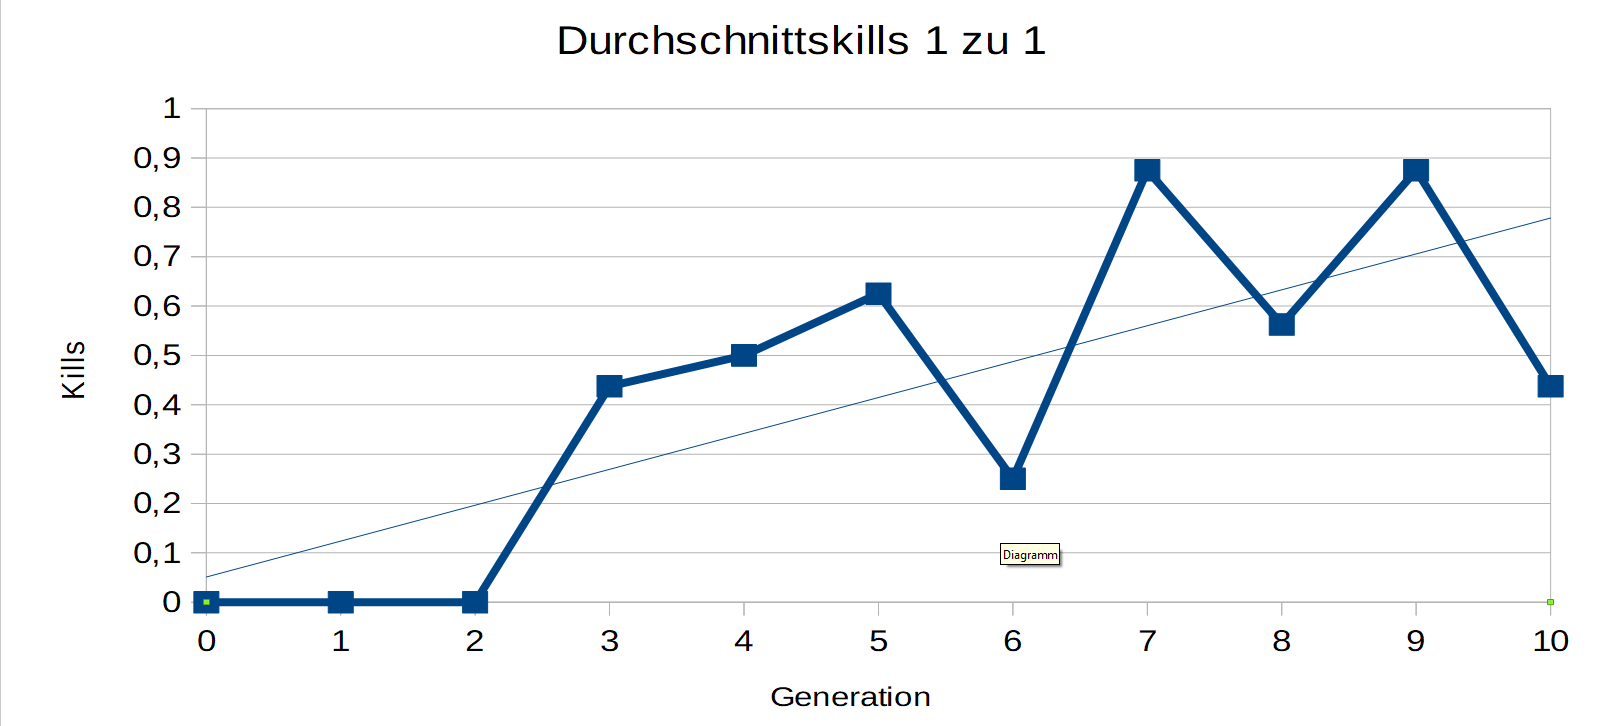
\includegraphics[width = \textwidth]{Durchschnittskills1zu1.png}
	\caption{figure1}
	\label{figure1}
\end{figure}\\
Diese Graphik zeigt die durchschnittlichen Kills des jeweiligen Individuums gegen die nullte Generation. Dabei ist die x-Achse die Generation, aus der das jeweilige Individuum stammt, und die y-Achse der Durchschnittswert, der gegen die nullte Generation erzielten Kills. Die Punkte sind dabei die Einzelwerte, während die Gerade eine lineare Regression aller Werte ist, also den Trend anzeigt.\\
Die Stagnation von der nullten bis zur zweiten Generation liegt höchstwahrscheinlich daran, dass das Abschießen von Gegnereinheiten erst durch eine Mutation erlernt werden musste. Ab der dritten Generation zeichnet sich ein Aufwärtstrend ab. Die Einbrüche innerhalb dessen sind der Fitnessfunktion geschuldet: Ein Individuum kann innerhalb einer Population besser sein als in einer anderen; schließlich muss man sich begegnen, um sich bekämpfen zu können. Trotzdem gehen wir davon aus, dass sich auf längere Sicht, sprich mehr Generationen, der Aufwärtstrend fortsetzen würde.\\
Wir sind bisher nicht auf Verluste eingegangen, da in dieser Variante die nullte Generation keinem Individuum Verluste zufügen konnte.

\section{Variante2: 1zu2}
Diese Variante bewertet verwehrte gegnerische Einheiten doppelt so schwer wie verlorene eigene Einheiten. Die Motivation dieser Variante war einen aggressiveren Spielstil zu bevorzugen, damit aktive Strategien extrinsisch motiviert werden.
\begin{figure}[h]
	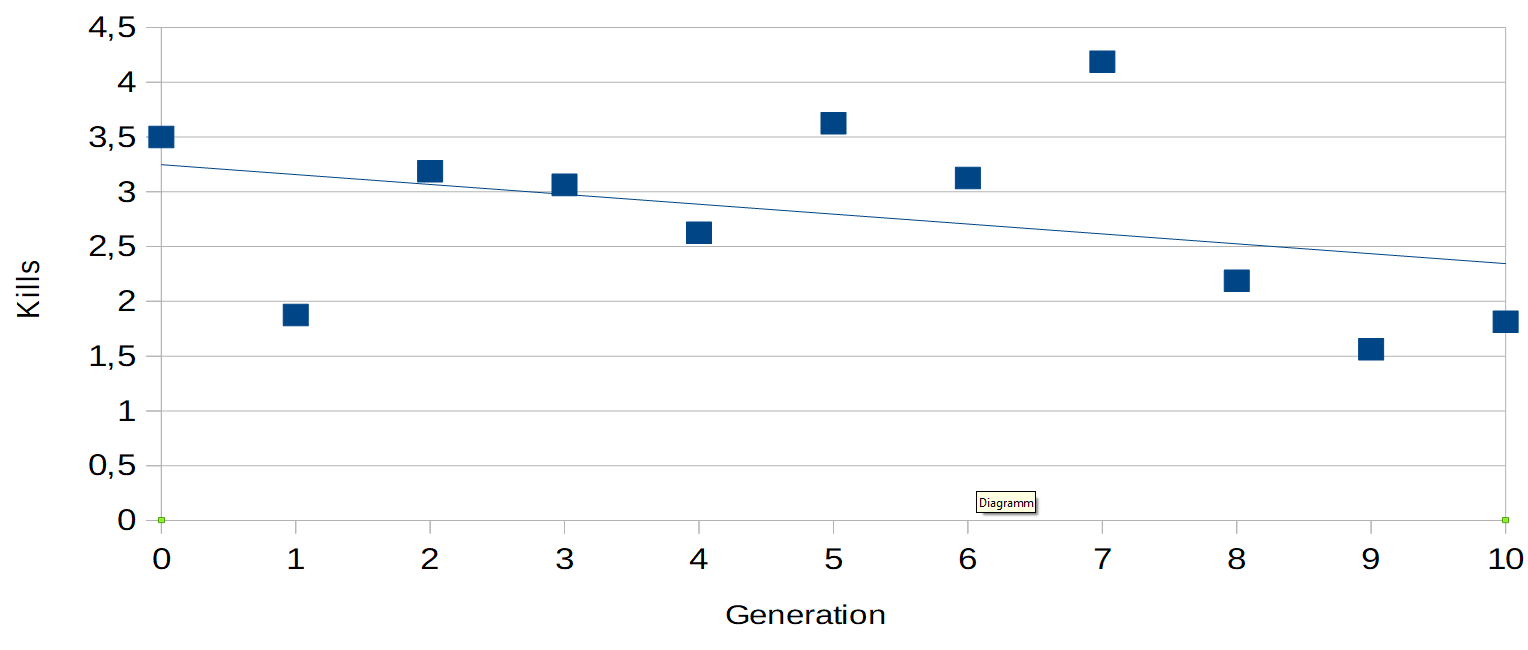
\includegraphics[width = \textwidth]{Durchschnittskills1zu2.png}
	\caption{figure2}
	\label{figure2}
\end{figure}\\
\begin{figure}[h]
	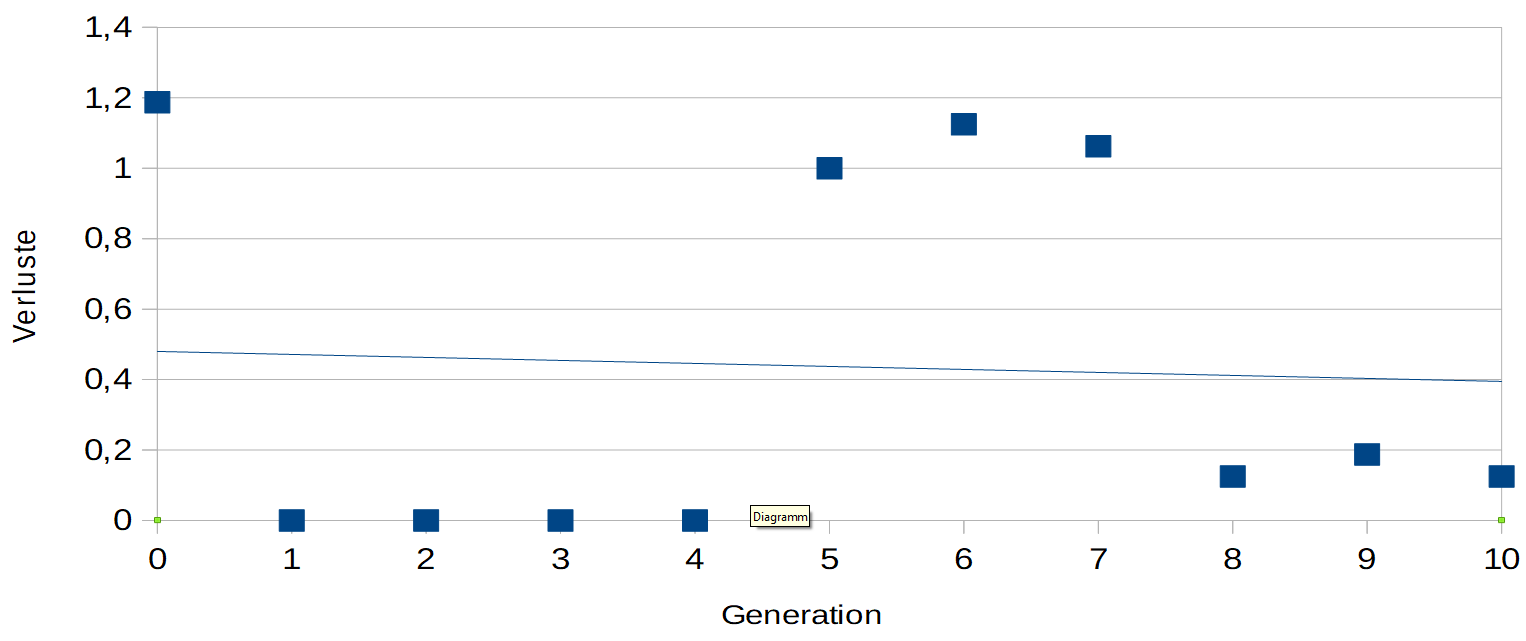
\includegraphics[width = \textwidth]{Durchschnittsverluste1zu2.png}
	\caption{figure3}
	\label{figure3}
\end{figure}\\
Die obere Graphik zeigt die durchschnittlichen Kills des jeweiligen Individuums gegen die nullte Generation, die untere zeigt die durchschnittlichen Verluste. Die Achsen entsprechen der ersten Abbildung (\ref{figure1}).\\
Beide Graphiken haben gemeinsam, dass sich kein klarer Gesammttrend herauslesen lässt. Allerdings ist klar zu erkennen, dass bei dieser Variante die nullte Generation zufälligerweise wesentlich aggressiver als andere nullte Generationen ist. Diese Aggressivität bleibt bis zur siebten Generation deutlich sichtbar. Wahrscheinlich ringt diese Variante um eine Balance zwischen aggressiver Vernichtung des Gegners und Minimierung eigener Verluste. Dies hängt natürlich eng mit der generell aggressiven Grundstimmung der Population zusammen. Da Kills, in dieser Variante, mehr zählen als Verluste geht diese aggressive Grundstimmung auch nicht verloren. Ab der achten Generation scheint die Vermeidung von Verlusten überhand über das Erzielen von Kills zu gewinnen, wodurch sich die Aggressivität senkt. Dies hat zur Folge, dass zwar die Kills zurückgehen jedoch die Verluste deutlich stärker abnehmen.

\section{Variante3: 0zu1}
Diese Variante bewertet nur verwehrte gegnerische Einheiten und ignoriert verlorene eigene Einheiten. Die Motivation dieser Variante war einen aggressiven Spielstil zu forcieren, um damit eine hohe Aktivität zu schaffen.
\begin{figure}[h]
	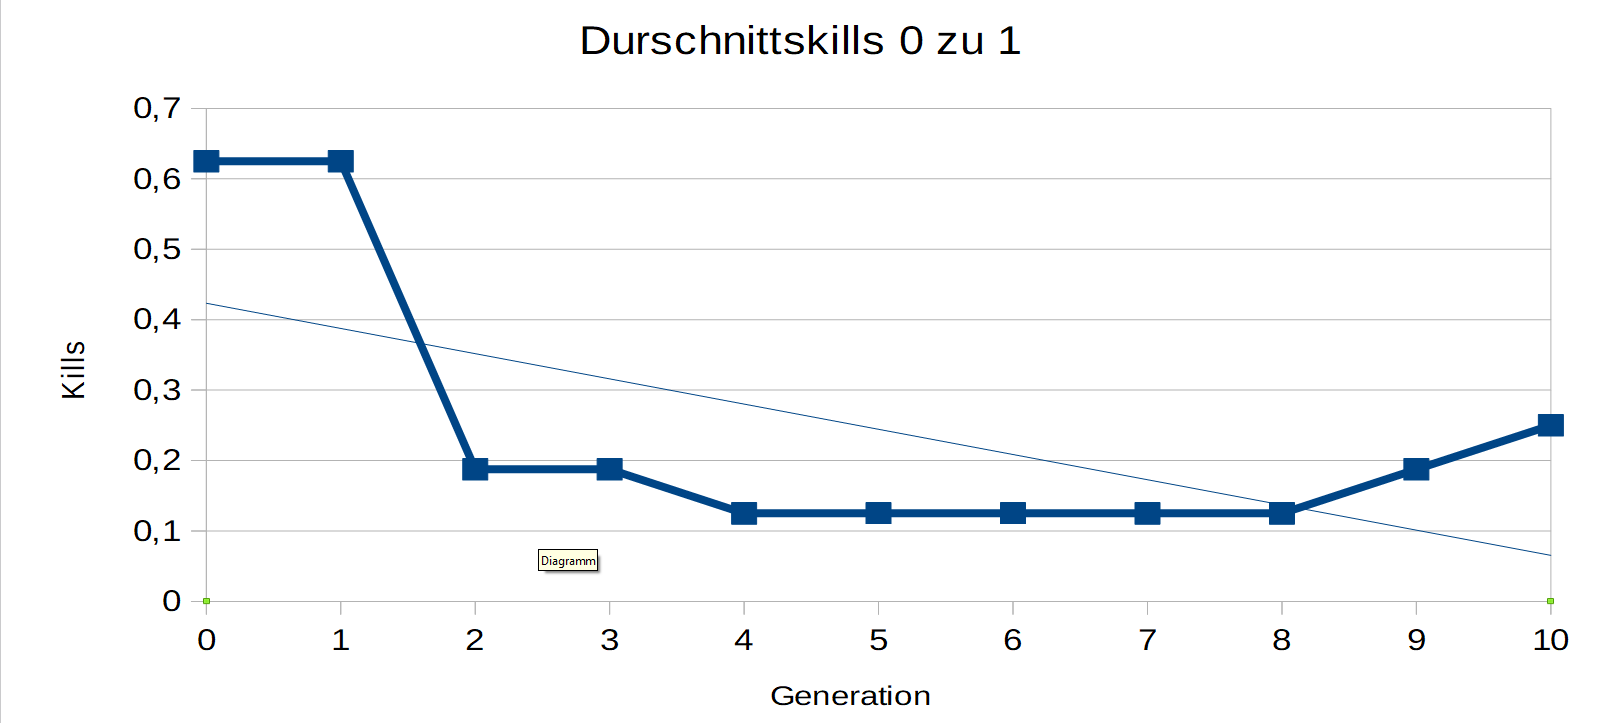
\includegraphics[width = \textwidth]{Durchschnittskills0zu1.png}
	\caption{figure4}
	\label{figure4}
\end{figure}\\
Die obere Graphik zeigt die durchschnittlichen Kills des jeweiligen Individuums gegen die nullte Generation. Die Achsen entsprechen der ersten Abbildung (\ref{figure1}).\\
Wieder haben wir keine Grafik zu Verlusten, weil es keine gab.\\
Das erste, was an dieser Grafik auffällt, ist der starke Abfall nach der ersten Generation. Dies ist ein Indikator dafür, dass sich zuerst ein passiver Spielstil durchsetzen konnte. Da für uns auch am Fitnesswert nicht abzusehen ist, ob dies tatsächlich zur Vermeidung von Verlusten geführt hat, ist diese Entwicklung schwer einzuschätzen. Jedenfalls sind passive Individuen auch schwieriger anzugreifen.\\
Ab der neunten Generation setzt dann ein Aufwärtstrend ein. Bei dieser Variante ist klar zu erkennen, dass ohne Abstrafung von Verlusten sich passive Individuen unerwartet gut in der Population halten können.

\chapter{Conclusion}
\label{Conclusion}

Lorem ipsum dolor sit amet, consetetur sadipscing elitr, sed diam nonumy eirmod tempor invidunt ut labore et dolore magna aliquyam erat, sed diam voluptua.
At vero eos et accusam et justo duo dolores et ea rebum.
Stet clita kasd gubergren, no sea takimata sanctus est Lorem ipsum dolor sit amet.

\bibliographystyle{alpha}
\bibliography{literatur}

\appendix
\appendixpage

[Spring] https://springrts.com/
[Unity] https://unity3d.com/
[NN-Bib] http://franck.fleurey.free.fr/NeuralNetwork/

\chapter{Chapter}

Lorem ipsum dolor sit amet, consetetur sadipscing elitr, sed diam nonumy eirmod tempor invidunt ut labore et dolore magna aliquyam erat, sed diam voluptua.
At vero eos et accusam et justo duo dolores et ea rebum.
Stet clita kasd gubergren, no sea takimata sanctus est Lorem ipsum dolor sit amet.

\listoffigures

\lstlistoflistings

\listoftables

\chapter*{}

\thispagestyle{empty}

\section*{Eidesstattliche Versicherung}

\begin{otherlanguage}{ngerman}
Hiermit versichere ich an Eides statt, dass ich die vorliegende Arbeit im Studiengang XXX selbstständig verfasst und keine anderen als die angegebenen Hilfsmittel -- insbesondere keine im Quellenverzeichnis nicht benannten Internet-Quellen -- benutzt habe.
Alle Stellen, die wörtlich oder sinngemäß aus Veröffentlichungen entnommen wurden, sind als solche kenntlich gemacht.
Ich versichere weiterhin, dass ich die Arbeit vorher nicht in einem anderen Prüfungsverfahren eingereicht habe und die eingereichte schriftliche Fassung der auf dem elektronischen Speichermedium entspricht.
\end{otherlanguage}

\vspace{1cm}

\begin{center}
\begin{tabular}{ll}
	\rule{0.35\textwidth}{0.4pt} & \rule{0.55\textwidth}{0.4pt} \\
	Ort, Datum & Unterschrift
\end{tabular}
\end{center}

\vfill

\section*{Veröffentlichung}

\begin{otherlanguage}{ngerman}
Ich bin damit einverstanden, dass meine Arbeit in den Bestand der Bibliothek des Fachbereichs Informatik eingestellt wird.
\end{otherlanguage}

\vspace{1cm}

\begin{center}
\begin{tabular}{ll}
	\rule{0.35\textwidth}{0.4pt} & \rule{0.55\textwidth}{0.4pt} \\
	Ort, Datum & Unterschrift
\end{tabular}
\end{center}

\end{document}
